\documentclass[11pt,a4paper,fleqn]{article}
\usepackage{graphicx} 
\usepackage{multirow}
\usepackage{hhline}
\begin{document}
\textbf{CS6140 Machine Learning Fall 2014 Homework 2, Wei Luo }\\
\\
\textbf{PROBLEM 1}\\
\\
 \textbf{B)} Training and testing performance across all four learning algorithms is: \\
 
 \hskip-2cm
 \begin{tabular}{|l|l|l|l|l|}
\hline
 &Decision or &Linear Regression &Linear Regression&LogisticRegression\\
 &Regression Tree&(Normal Equations)&(Gradient Descent)&(Gradeint Descent)\\
\hline
Spambase&Train ACC: 0.91&Train ACC: 0.92&Train ACC: 0.91&Train ACC: 0.92\\
&Test ACC: 0.90&Test ACC: 0.88&Test ACC: 0.90&Test ACC: 0.91\\
\hline
Housing&Train MSE: 26.49&Train MSE: 22.08&Train MSE: 22.13&N/A.\\
 &Test MSE: 24.28&Test MSE: 22.63&Test MSE: 22.58&\\
\hline
\end{tabular}\\
\\ \\
 \textbf{C)} \\
 Confusion Matrix for Decision Tree:\\ \\
\begin{tabular}{cc|c|c|}
\multicolumn{2}{c}{}&\multicolumn{2}{c}{Prediction}\\
\multicolumn{2}{c}{}&\multicolumn{1}{c}{1}&\multicolumn{1}{c}{0}\\
\hhline{~~--}
\multirow{2}{*}{Label}
&1&152&29\\
\hhline{~~--}
&0&14&264\\
\hhline{~~--}
\end{tabular}\\ \\
 Confusion Matrix for Linear Regression:\\ \\
\begin{tabular}{cc|c|c|}
\multicolumn{2}{c}{}&\multicolumn{2}{c}{Prediction}\\
\multicolumn{2}{c}{}&\multicolumn{1}{c}{1}&\multicolumn{1}{c}{0}\\
\hhline{~~--}
\multirow{2}{*}{Label}
&1&162&19\\
\hhline{~~--}
&0&22&256\\
\hhline{~~--}
\end{tabular}\\ \\
 Confusion Matrix for Logistic Regression:\\ \\
\begin{tabular}{cc|c|c|}
\multicolumn{2}{c}{}&\multicolumn{2}{c}{Prediction}\\
\multicolumn{2}{c}{}&\multicolumn{1}{c}{1}&\multicolumn{1}{c}{0}\\
\hhline{~~--}
\multirow{2}{*}{Label}
&1&154&27\\
\hhline{~~--}
&0&10&268\\
\hhline{~~--}
\end{tabular}\\ \\
\newpage \noindent
\textbf{D)} \\
ROC curve for Linear Regression:\\
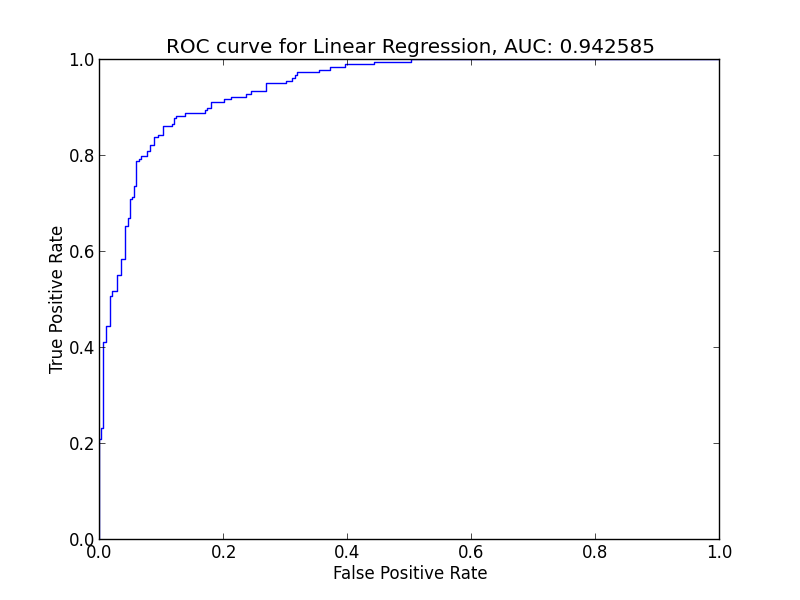
\includegraphics[scale=0.6]{ROC_Linear_Regression.png}\\
ROC curve for Logistic Regression:\\
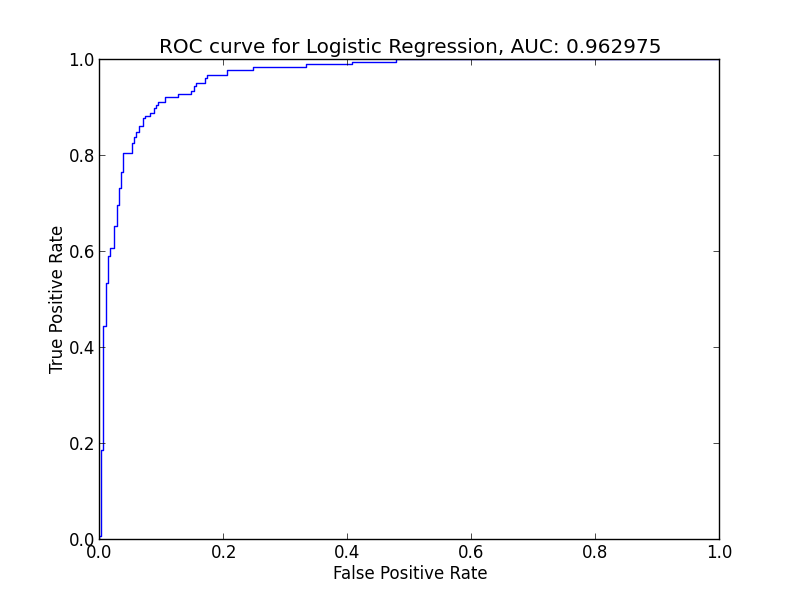
\includegraphics[scale=0.6]{ROC_Logistic_Regression.png}\\
\newpage \noindent
\textbf{PROBLEM 2}\\ \\
Iteration 1, total\_mistake 136\\
Iteration 2, total\_mistake 68\\
Iteration 3, total\_mistake 50\\
Iteration 4, total\_mistake 22\\
Iteration 5, total\_mistake 21\\
Iteration 6, total\_mistake 34\\
Iteration 7, total\_mistake 25\\
Iteration 8, total\_mistake 0\\
Classifier weights:\indent-14.\indent2.52873259\indent5.70717051\indent8.52231457\indent11.32560723\\
Normalized with threshold: \indent0.18062376\indent0.40765504\indent0.60873676\indent0.80897195\\
\\ \\
\textbf{PROBLEM 3}\\ \\
\end{document}